\section{CTCLProcessor  Class Reference}
\label{classCTCLProcessor}\index{CTCLProcessor@{CTCLProcessor}}
{\tt \#include $<$TCLProcessor.h$>$}

Inheritance diagram for CTCLProcessor::\begin{figure}[H]
\begin{center}
\leavevmode
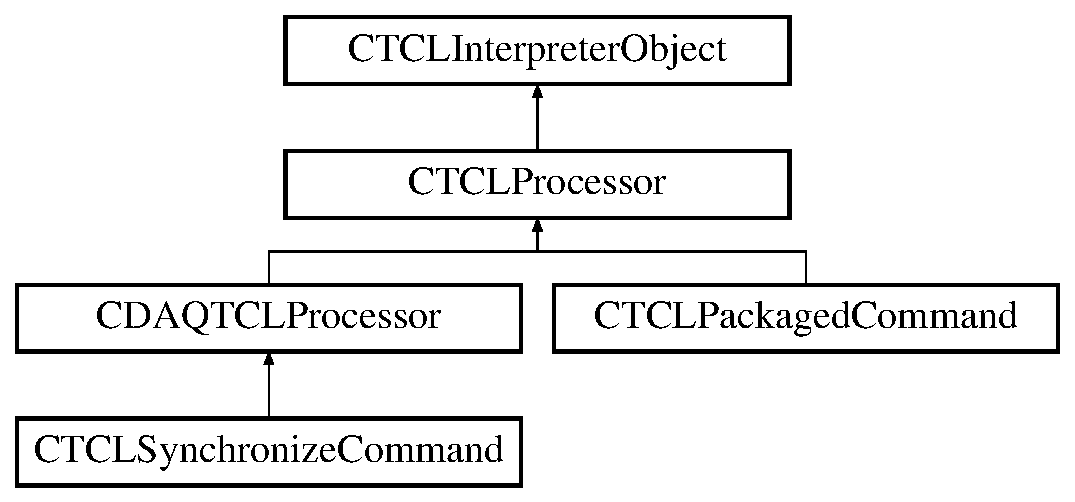
\includegraphics[height=4cm]{classCTCLProcessor}
\end{center}
\end{figure}
\subsection*{Public Methods}
\begin{CompactItemize}
\item 
{\bf CTCLProcessor} (const std::string \&s\-Command, {\bf CTCLInterpreter} $\ast$p\-Interp)
\item 
{\bf CTCLProcessor} (const char $\ast$p\-Command, {\bf CTCLInterpreter} $\ast$p\-Interp)
\item 
virtual {\bf $\sim$CTCLProcessor} ()
\item 
int {\bf operator==} (const CTCLProcessor \&a\-CTCLProcessor) const
\item 
std::string {\bf get\-Command\-Name} () const
\item 
{\bf TCLInterpreter\-Iterator} {\bf begin} ()
\item 
{\bf TCLInterpreter\-Iterator} {\bf end} ()
\item 
virtual int {\bf operator()} ({\bf CTCLInterpreter} \&r\-Interpreter, {\bf CTCLResult} \&r\-Result, int n\-Arguments, char $\ast$p\-Arguments[$\,$])=0
\item 
virtual void {\bf On\-Delete} ()
\item 
int {\bf Parse\-Int} (const char $\ast$p\-String, int $\ast$p\-Integer)
\item 
int {\bf Parse\-Int} (const std::string \&r\-String, int $\ast$p\-Integer)
\item 
int {\bf Parse\-Double} (const char $\ast$p\-String, double $\ast$p\-Double)
\item 
int {\bf Parse\-Double} (const std::string \&r\-String, double $\ast$p\-Double)
\item 
int {\bf Parse\-Boolean} (const char $\ast$p\-String, {\bf Bool\_\-t} $\ast$p\-Boolean)
\item 
int {\bf Parse\-Boolean} (const std::string \&r\-String, {\bf Bool\_\-t} $\ast$p\-Boolean)
\item 
virtual void {\bf Register} ()
\item 
int {\bf Unregister} ()
\item 
void {\bf Unregister\-All} ()
\end{CompactItemize}
\subsection*{Static Public Methods}
\begin{CompactItemize}
\item 
std::string {\bf Concatenate\-Parameters} (int n\-Arguments, char $\ast$p\-Arguments[$\,$])
\item 
int {\bf Eval\-Relay} (Client\-Data p\-Data, Tcl\_\-Interp $\ast$p\-Interp, int Argc, char $\ast$Argv[$\,$])
\item 
void {\bf Delete\-Relay} (Client\-Data p\-Object)
\item 
int {\bf Match\-Keyword} (vector$<$ string $>$ \&Match\-Table, const string \&r\-Value, int No\-Match=-1)
\end{CompactItemize}
\subsection*{Protected Methods}
\begin{CompactItemize}
\item 
void {\bf set\-Command\-Name} (const std::string \&am\_\-s\-Command\-Name)
\item 
void {\bf set\-Registered\-On} (const std::vector$<$ {\bf CTCLInterpreter} $\ast$ $>$ \&am\_\-v\-Registered\-On)
\item 
void {\bf Add\-Registered\-On\-Current} ()
\end{CompactItemize}
\subsection*{Private Methods}
\begin{CompactItemize}
\item 
{\bf CTCLProcessor} (const CTCLProcessor \&a\-CTCLProcessor)
\item 
CTCLProcessor \& {\bf operator=} (const CTCLProcessor \&a\-CTCLProcessor)
\end{CompactItemize}
\subsection*{Private Attributes}
\begin{CompactItemize}
\item 
std::string {\bf m\_\-s\-Command\-Name}
\item 
{\bf TCLInterpreter\-List} {\bf m\_\-v\-Registered\-On}
\end{CompactItemize}


\subsection{Constructor \& Destructor Documentation}
\index{CTCLProcessor@{CTCLProcessor}!CTCLProcessor@{CTCLProcessor}}
\index{CTCLProcessor@{CTCLProcessor}!CTCLProcessor@{CTCLProcessor}}
\subsubsection{\setlength{\rightskip}{0pt plus 5cm}CTCLProcessor::CTCLProcessor (const std::string \& {\em s\-Command}, {\bf CTCLInterpreter} $\ast$ {\em p\-Interp})}\label{classCTCLProcessor_a0}




Definition at line 323 of file TCLProcessor.cpp.

References m\_\-s\-Command\-Name.\index{CTCLProcessor@{CTCLProcessor}!CTCLProcessor@{CTCLProcessor}}
\index{CTCLProcessor@{CTCLProcessor}!CTCLProcessor@{CTCLProcessor}}
\subsubsection{\setlength{\rightskip}{0pt plus 5cm}CTCLProcessor::CTCLProcessor (const char $\ast$ {\em p\-Command}, {\bf CTCLInterpreter} $\ast$ {\em p\-Interp})}\label{classCTCLProcessor_a1}




Definition at line 330 of file TCLProcessor.cpp.

References m\_\-s\-Command\-Name.\index{CTCLProcessor@{CTCLProcessor}!~CTCLProcessor@{$\sim$CTCLProcessor}}
\index{~CTCLProcessor@{$\sim$CTCLProcessor}!CTCLProcessor@{CTCLProcessor}}
\subsubsection{\setlength{\rightskip}{0pt plus 5cm}virtual CTCLProcessor::$\sim$CTCLProcessor ()\hspace{0.3cm}{\tt  [inline, virtual]}}\label{classCTCLProcessor_a2}




Definition at line 334 of file TCLProcessor.h.

References Unregister\-All().\index{CTCLProcessor@{CTCLProcessor}!CTCLProcessor@{CTCLProcessor}}
\index{CTCLProcessor@{CTCLProcessor}!CTCLProcessor@{CTCLProcessor}}
\subsubsection{\setlength{\rightskip}{0pt plus 5cm}CTCLProcessor::CTCLProcessor (const CTCLProcessor \& {\em a\-CTCLProcessor})\hspace{0.3cm}{\tt  [private]}}\label{classCTCLProcessor_c0}




\subsection{Member Function Documentation}
\index{CTCLProcessor@{CTCLProcessor}!AddRegisteredOnCurrent@{AddRegisteredOnCurrent}}
\index{AddRegisteredOnCurrent@{AddRegisteredOnCurrent}!CTCLProcessor@{CTCLProcessor}}
\subsubsection{\setlength{\rightskip}{0pt plus 5cm}void CTCLProcessor::Add\-Registered\-On\-Current ()\hspace{0.3cm}{\tt  [inline, protected]}}\label{classCTCLProcessor_b2}




Definition at line 380 of file TCLProcessor.h.

References CTCLInterpreter\-Object::Assert\-If\-Not\-Bound(), and m\_\-v\-Registered\-On.

Referenced by CDAQTCLProcessor::Register().\index{CTCLProcessor@{CTCLProcessor}!begin@{begin}}
\index{begin@{begin}!CTCLProcessor@{CTCLProcessor}}
\subsubsection{\setlength{\rightskip}{0pt plus 5cm}{\bf TCLInterpreter\-Iterator} CTCLProcessor::begin ()\hspace{0.3cm}{\tt  [inline]}}\label{classCTCLProcessor_a5}




Definition at line 364 of file TCLProcessor.h.

References m\_\-v\-Registered\-On, and TCLInterpreter\-Iterator.

Referenced by Delete\-Relay(), and Eval\-Relay().\index{CTCLProcessor@{CTCLProcessor}!ConcatenateParameters@{ConcatenateParameters}}
\index{ConcatenateParameters@{ConcatenateParameters}!CTCLProcessor@{CTCLProcessor}}
\subsubsection{\setlength{\rightskip}{0pt plus 5cm}std::string CTCLProcessor::Concatenate\-Parameters (int {\em n\-Arguments}, char $\ast$ {\em p\-Arguments}[$\,$])\hspace{0.3cm}{\tt  [static]}}\label{classCTCLProcessor_d0}




Definition at line 346 of file TCLProcessor.cpp.\index{CTCLProcessor@{CTCLProcessor}!DeleteRelay@{DeleteRelay}}
\index{DeleteRelay@{DeleteRelay}!CTCLProcessor@{CTCLProcessor}}
\subsubsection{\setlength{\rightskip}{0pt plus 5cm}void CTCLProcessor::Delete\-Relay (Client\-Data {\em p\-Object})\hspace{0.3cm}{\tt  [static]}}\label{classCTCLProcessor_d2}




Reimplemented in {\bf CDAQTCLProcessor} {\rm (p.\,\pageref{classCDAQTCLProcessor_f1})}.

Definition at line 489 of file TCLProcessor.cpp.

References begin(), CTCLInterpreter\-Object::Bind(), end(), CTCLInterpreter::get\-Interpreter(), CTCLInterpreter\-Object::get\-Interpreter(), m\_\-v\-Registered\-On, On\-Delete(), and TCLInterpreter\-Iterator.

Referenced by CDAQTCLProcessor::Delete\-Relay(), and Register().\index{CTCLProcessor@{CTCLProcessor}!end@{end}}
\index{end@{end}!CTCLProcessor@{CTCLProcessor}}
\subsubsection{\setlength{\rightskip}{0pt plus 5cm}{\bf TCLInterpreter\-Iterator} CTCLProcessor::end ()\hspace{0.3cm}{\tt  [inline]}}\label{classCTCLProcessor_a6}




Definition at line 367 of file TCLProcessor.h.

References m\_\-v\-Registered\-On, and TCLInterpreter\-Iterator.

Referenced by Delete\-Relay(), and Eval\-Relay().\index{CTCLProcessor@{CTCLProcessor}!EvalRelay@{EvalRelay}}
\index{EvalRelay@{EvalRelay}!CTCLProcessor@{CTCLProcessor}}
\subsubsection{\setlength{\rightskip}{0pt plus 5cm}int CTCLProcessor::Eval\-Relay (Client\-Data {\em p\-Data}, Tcl\_\-Interp $\ast$ {\em p\-Interp}, int {\em Argc}, char $\ast$ {\em Argv}[$\,$])\hspace{0.3cm}{\tt  [static]}}\label{classCTCLProcessor_d1}




Definition at line 387 of file TCLProcessor.cpp.

References begin(), CTCLInterpreter\-Object::Bind(), end(), CTCLInterpreter::get\-Interpreter(), CTCLInterpreter\-Object::get\-Interpreter(), and TCLInterpreter\-Iterator.

Referenced by CDAQTCLProcessor::Eval\-Relay(), and Register().\index{CTCLProcessor@{CTCLProcessor}!getCommandName@{getCommandName}}
\index{getCommandName@{getCommandName}!CTCLProcessor@{CTCLProcessor}}
\subsubsection{\setlength{\rightskip}{0pt plus 5cm}std::string CTCLProcessor::get\-Command\-Name () const\hspace{0.3cm}{\tt  [inline]}}\label{classCTCLProcessor_a4}




Definition at line 360 of file TCLProcessor.h.

References m\_\-s\-Command\-Name.

Referenced by CDAQTCLProcessor::Register().\index{CTCLProcessor@{CTCLProcessor}!MatchKeyword@{MatchKeyword}}
\index{MatchKeyword@{MatchKeyword}!CTCLProcessor@{CTCLProcessor}}
\subsubsection{\setlength{\rightskip}{0pt plus 5cm}int CTCLProcessor::Match\-Keyword (vector$<$ string $>$ \& {\em Match\-Table}, const string \& {\em r\-Value}, int {\em No\-Match} = -1)\hspace{0.3cm}{\tt  [static]}}\label{classCTCLProcessor_d3}




Definition at line 706 of file TCLProcessor.cpp.\index{CTCLProcessor@{CTCLProcessor}!OnDelete@{OnDelete}}
\index{OnDelete@{OnDelete}!CTCLProcessor@{CTCLProcessor}}
\subsubsection{\setlength{\rightskip}{0pt plus 5cm}void CTCLProcessor::On\-Delete ()\hspace{0.3cm}{\tt  [virtual]}}\label{classCTCLProcessor_a8}




Definition at line 460 of file TCLProcessor.cpp.

Referenced by Delete\-Relay().\index{CTCLProcessor@{CTCLProcessor}!operator()@{operator()}}
\index{operator()@{operator()}!CTCLProcessor@{CTCLProcessor}}
\subsubsection{\setlength{\rightskip}{0pt plus 5cm}virtual int CTCLProcessor::operator() ({\bf CTCLInterpreter} \& {\em r\-Interpreter}, {\bf CTCLResult} \& {\em r\-Result}, int {\em n\-Arguments}, char $\ast$ {\em p\-Arguments}[$\,$])\hspace{0.3cm}{\tt  [pure virtual]}}\label{classCTCLProcessor_a7}




Implemented in {\bf CTCLSynchronize\-Command} {\rm (p.\,\pageref{classCTCLSynchronizeCommand_a3})}.\index{CTCLProcessor@{CTCLProcessor}!operator=@{operator=}}
\index{operator=@{operator=}!CTCLProcessor@{CTCLProcessor}}
\subsubsection{\setlength{\rightskip}{0pt plus 5cm}CTCLProcessor\& CTCLProcessor::operator= (const CTCLProcessor \& {\em a\-CTCLProcessor})\hspace{0.3cm}{\tt  [private]}}\label{classCTCLProcessor_c1}


\index{CTCLProcessor@{CTCLProcessor}!operator==@{operator==}}
\index{operator==@{operator==}!CTCLProcessor@{CTCLProcessor}}
\subsubsection{\setlength{\rightskip}{0pt plus 5cm}int CTCLProcessor::operator== (const CTCLProcessor \& {\em a\-CTCLProcessor}) const\hspace{0.3cm}{\tt  [inline]}}\label{classCTCLProcessor_a3}




Definition at line 350 of file TCLProcessor.h.

References m\_\-s\-Command\-Name, m\_\-v\-Registered\-On, and CTCLInterpreter\-Object::operator==().

Referenced by CTCLPackaged\-Command::operator==(), CTCLSynchronize\-Command::operator==(), and CDAQTCLProcessor::operator==().\index{CTCLProcessor@{CTCLProcessor}!ParseBoolean@{ParseBoolean}}
\index{ParseBoolean@{ParseBoolean}!CTCLProcessor@{CTCLProcessor}}
\subsubsection{\setlength{\rightskip}{0pt plus 5cm}int CTCLProcessor::Parse\-Boolean (const std::string \& {\em r\-String}, {\bf Bool\_\-t} $\ast$ {\em p\-Boolean})\hspace{0.3cm}{\tt  [inline]}}\label{classCTCLProcessor_a14}




Definition at line 411 of file TCLProcessor.h.

References Bool\_\-t, and Parse\-Boolean().\index{CTCLProcessor@{CTCLProcessor}!ParseBoolean@{ParseBoolean}}
\index{ParseBoolean@{ParseBoolean}!CTCLProcessor@{CTCLProcessor}}
\subsubsection{\setlength{\rightskip}{0pt plus 5cm}int CTCLProcessor::Parse\-Boolean (const char $\ast$ {\em p\-String}, {\bf Bool\_\-t} $\ast$ {\em p\-Boolean})}\label{classCTCLProcessor_a13}




Definition at line 604 of file TCLProcessor.cpp.

References Bool\_\-t, CTCLInterpreter::get\-Interpreter(), and CTCLInterpreter\-Object::get\-Interpreter().

Referenced by Parse\-Boolean().\index{CTCLProcessor@{CTCLProcessor}!ParseDouble@{ParseDouble}}
\index{ParseDouble@{ParseDouble}!CTCLProcessor@{CTCLProcessor}}
\subsubsection{\setlength{\rightskip}{0pt plus 5cm}int CTCLProcessor::Parse\-Double (const std::string \& {\em r\-String}, double $\ast$ {\em p\-Double})\hspace{0.3cm}{\tt  [inline]}}\label{classCTCLProcessor_a12}




Definition at line 406 of file TCLProcessor.h.

References Parse\-Double().\index{CTCLProcessor@{CTCLProcessor}!ParseDouble@{ParseDouble}}
\index{ParseDouble@{ParseDouble}!CTCLProcessor@{CTCLProcessor}}
\subsubsection{\setlength{\rightskip}{0pt plus 5cm}int CTCLProcessor::Parse\-Double (const char $\ast$ {\em p\-String}, double $\ast$ {\em p\-Double})}\label{classCTCLProcessor_a11}




Definition at line 572 of file TCLProcessor.cpp.

References CTCLInterpreter::get\-Interpreter(), and CTCLInterpreter\-Object::get\-Interpreter().

Referenced by Parse\-Double().\index{CTCLProcessor@{CTCLProcessor}!ParseInt@{ParseInt}}
\index{ParseInt@{ParseInt}!CTCLProcessor@{CTCLProcessor}}
\subsubsection{\setlength{\rightskip}{0pt plus 5cm}int CTCLProcessor::Parse\-Int (const std::string \& {\em r\-String}, int $\ast$ {\em p\-Integer})\hspace{0.3cm}{\tt  [inline]}}\label{classCTCLProcessor_a10}




Definition at line 401 of file TCLProcessor.h.

References Parse\-Int().\index{CTCLProcessor@{CTCLProcessor}!ParseInt@{ParseInt}}
\index{ParseInt@{ParseInt}!CTCLProcessor@{CTCLProcessor}}
\subsubsection{\setlength{\rightskip}{0pt plus 5cm}int CTCLProcessor::Parse\-Int (const char $\ast$ {\em p\-String}, int $\ast$ {\em p\-Integer})}\label{classCTCLProcessor_a9}




Definition at line 533 of file TCLProcessor.cpp.

References CTCLInterpreter::get\-Interpreter(), and CTCLInterpreter\-Object::get\-Interpreter().

Referenced by Parse\-Int().\index{CTCLProcessor@{CTCLProcessor}!Register@{Register}}
\index{Register@{Register}!CTCLProcessor@{CTCLProcessor}}
\subsubsection{\setlength{\rightskip}{0pt plus 5cm}void CTCLProcessor::Register ()\hspace{0.3cm}{\tt  [virtual]}}\label{classCTCLProcessor_a15}




Reimplemented in {\bf CDAQTCLProcessor} {\rm (p.\,\pageref{classCDAQTCLProcessor_a4})}.

Definition at line 642 of file TCLProcessor.cpp.

References CTCLInterpreter::Add\-Command(), CTCLInterpreter\-Object::Assert\-If\-Not\-Bound(), Delete\-Relay(), Eval\-Relay(), m\_\-s\-Command\-Name, and m\_\-v\-Registered\-On.\index{CTCLProcessor@{CTCLProcessor}!setCommandName@{setCommandName}}
\index{setCommandName@{setCommandName}!CTCLProcessor@{CTCLProcessor}}
\subsubsection{\setlength{\rightskip}{0pt plus 5cm}void CTCLProcessor::set\-Command\-Name (const std::string \& {\em am\_\-s\-Command\-Name})\hspace{0.3cm}{\tt  [inline, protected]}}\label{classCTCLProcessor_b0}




Definition at line 374 of file TCLProcessor.h.

References m\_\-s\-Command\-Name.\index{CTCLProcessor@{CTCLProcessor}!setRegisteredOn@{setRegisteredOn}}
\index{setRegisteredOn@{setRegisteredOn}!CTCLProcessor@{CTCLProcessor}}
\subsubsection{\setlength{\rightskip}{0pt plus 5cm}void CTCLProcessor::set\-Registered\-On (const std::vector$<$ {\bf CTCLInterpreter} $\ast$ $>$ \& {\em am\_\-v\-Registered\-On})\hspace{0.3cm}{\tt  [inline, protected]}}\label{classCTCLProcessor_b1}




Definition at line 377 of file TCLProcessor.h.

References m\_\-v\-Registered\-On.\index{CTCLProcessor@{CTCLProcessor}!Unregister@{Unregister}}
\index{Unregister@{Unregister}!CTCLProcessor@{CTCLProcessor}}
\subsubsection{\setlength{\rightskip}{0pt plus 5cm}int CTCLProcessor::Unregister ()}\label{classCTCLProcessor_a16}




Definition at line 663 of file TCLProcessor.cpp.

References CTCLInterpreter\-Object::Assert\-If\-Not\-Bound(), m\_\-s\-Command\-Name, and CTCLInterpreter::Unregister\-Command().

Referenced by Unregister\-All().\index{CTCLProcessor@{CTCLProcessor}!UnregisterAll@{UnregisterAll}}
\index{UnregisterAll@{UnregisterAll}!CTCLProcessor@{CTCLProcessor}}
\subsubsection{\setlength{\rightskip}{0pt plus 5cm}void CTCLProcessor::Unregister\-All ()}\label{classCTCLProcessor_a17}




Definition at line 684 of file TCLProcessor.cpp.

References CTCLInterpreter\-Object::Bind(), CTCLInterpreter\-Object::get\-Interpreter(), m\_\-v\-Registered\-On, and Unregister().

Referenced by $\sim$CTCLProcessor().

\subsection{Member Data Documentation}
\index{CTCLProcessor@{CTCLProcessor}!m_sCommandName@{m\_\-sCommandName}}
\index{m_sCommandName@{m\_\-sCommandName}!CTCLProcessor@{CTCLProcessor}}
\subsubsection{\setlength{\rightskip}{0pt plus 5cm}std::string CTCLProcessor::m\_\-s\-Command\-Name\hspace{0.3cm}{\tt  [private]}}\label{classCTCLProcessor_o0}




Definition at line 324 of file TCLProcessor.h.

Referenced by CTCLProcessor(), get\-Command\-Name(), operator==(), Register(), set\-Command\-Name(), and Unregister().\index{CTCLProcessor@{CTCLProcessor}!m_vRegisteredOn@{m\_\-vRegisteredOn}}
\index{m_vRegisteredOn@{m\_\-vRegisteredOn}!CTCLProcessor@{CTCLProcessor}}
\subsubsection{\setlength{\rightskip}{0pt plus 5cm}{\bf TCLInterpreter\-List} CTCLProcessor::m\_\-v\-Registered\-On\hspace{0.3cm}{\tt  [private]}}\label{classCTCLProcessor_o1}




Definition at line 325 of file TCLProcessor.h.

Referenced by Add\-Registered\-On\-Current(), begin(), Delete\-Relay(), end(), operator==(), Register(), set\-Registered\-On(), and Unregister\-All().

The documentation for this class was generated from the following files:\begin{CompactItemize}
\item 
{\bf TCLProcessor.h}\item 
{\bf TCLProcessor.cpp}\end{CompactItemize}
